%=====================================================================
%  Wave Function of the Void — v6 (Final revision)
%  Andrei Preece and Boris Batenin, Berlin 2026
%
%  Changes from v5:
%  (A) Proposition 7.3 reformulated via Raychaudhuri equation
%  (B) Softened w_eff → −1 claim to parametrisation-fitting language
%  (C) Curvature-term asymptotic remark in §8.2
%  (D) Golden-ratio remark moved to appendix as numerical curiosity
%  (E) Gauge-invariant definition of a via 3-volume added
%=====================================================================
\documentclass[12pt,a4paper]{article}

\usepackage[margin=2.5cm,headheight=15pt]{geometry}
\usepackage{amsmath,amssymb,amsfonts,amsthm}
\usepackage{mathrsfs}
\usepackage{physics}
\usepackage{braket}
\usepackage{graphicx}
\usepackage{tikz}
\usetikzlibrary{arrows.meta,calc,shapes.geometric,positioning,
                decorations.pathmorphing,patterns}
\usepackage{pgfplots}
\pgfplotsset{compat=1.18}
\usepackage{hyperref}
\hypersetup{colorlinks=true,
            linkcolor=blue!60!black,
            citecolor=blue!60!black,
            urlcolor=blue!60!black}
\usepackage{fancyhdr}
\usepackage[expansion=false]{microtype}
\usepackage{booktabs}
\usepackage{array}
\usepackage{caption}
\usepackage{enumitem}
\usepackage{xcolor}
\usepackage{tcolorbox}
\tcbuselibrary{theorems,skins,breakable}
\usepackage{mathtools}
\usepackage{bm}
\usepackage{setspace}
\usepackage[numbers,sort&compress]{natbib}

%--- Theorem environments -------------------------------------------
\theoremstyle{plain}
\newtheorem{theorem}{Theorem}[section]
\newtheorem{proposition}[theorem]{Proposition}
\newtheorem{lemma}[theorem]{Lemma}
\newtheorem{corollary}[theorem]{Corollary}

\theoremstyle{definition}
\newtheorem{definition}[theorem]{Definition}
\newtheorem{remark}[theorem]{Remark}
\newtheorem{assumption}[theorem]{Assumption}

%--- Custom commands ------------------------------------------------
\newcommand{\Hil}{\mathscr{H}}
\newcommand{\HilM}{\mathscr{H}_{\mathrm{m}}}
\newcommand{\HilV}{\mathscr{H}_{\mathrm{v}}}
\newcommand{\Psim}{\Psi_{\mathrm{m}}}
\newcommand{\Psiv}{\Psi_{\mathrm{v}}}
\newcommand{\Htot}{\hat{H}_{\mathrm{tot}}}
\newcommand{\Hm}{\hat{H}_{\mathrm{m}}}
\newcommand{\Hv}{\hat{H}_{\mathrm{v}}}
\newcommand{\Hgrav}{\hat{H}_{\mathrm{grav}}}
\newcommand{\Hint}{\hat{H}_{\mathrm{int}}}
\newcommand{\rhom}{\hat{\rho}_{\mathrm{m}}}
\newcommand{\rhov}{\hat{\rho}_{\mathrm{v}}}
\newcommand{\Mpl}{m_{\mathrm{Pl}}}
\newcommand{\lpl}{\ell_{\mathrm{Pl}}}
\newcommand{\omm}{\omega_{\mathrm{m}}}
\newcommand{\omv}{\omega_{\mathrm{v}}}
\newcommand{\Sent}{S_{\mathrm{ent}}}
\newcommand{\defeq}{\coloneqq}
\newcommand{\Sgap}{\Delta_{\mathrm{gap}}}
\newcommand{\Mth}{\mathcal{M}}
\newcommand{\Leff}{\Lambda_{\mathrm{eff}}}

%--- Boxes ----------------------------------------------------------
\newtcolorbox{keybox}[1][]{
  enhanced,colback=blue!4!white,colframe=blue!50!black,
  fonttitle=\bfseries,title=#1,breakable}

%--- Header ---------------------------------------------------------
\pagestyle{fancy}
\fancyhf{}
\fancyhead[L]{\small\itshape Wave Function of the Void}
\fancyhead[R]{\small\itshape A.~Preece, B.~Batenin}
\fancyfoot[C]{\thepage}
\renewcommand{\headrulewidth}{0.4pt}

%====================================================================
\begin{document}
\onehalfspacing

%--- Title block ----------------------------------------------------
\begin{center}
{\LARGE\bfseries Wave Function of the Void:\\[4pt]
Dual-Sector Quantum Cosmology on $S^3$,\\[4pt]
Emergent Time, Entropy, and Geometric Expansion}

\bigskip
{\large Andrei Preece and Boris Batenin}\\[4pt]
{\itshape Independent Researchers}\\[4pt]
{\small Berlin, Germany, 2026}

\bigskip\bigskip
\begin{minipage}{0.89\textwidth}
\small\setstretch{1.3}
\textbf{Abstract.}
We present a mathematically rigorous dual-sector quantum cosmology in which
the Hilbert space of the Universe factorises as
$\Hil = \HilM\otimes\HilV$, with $\HilV$ carrying a
\emph{Wave Function of the Void} $\Psiv$.
Starting from the full ADM action on a compact, orientable three-manifold,
we derive the void-extended Wheeler--DeWitt (WDW-V) constraint.
The void sector is modelled as a \emph{standard} (non-phantom)
harmonic-oscillator field with positive kinetic term and positive-definite
zero-point energy.
Entanglement between the matter and void sectors, generated by a minimal
bilinear coupling $\Hint \propto a^3\hat\phi_m^2\hat\phi_v^2$, drives a
monotonically increasing von~Neumann entropy $\Sent(a)$, providing a
first-principles derivation of the second law of thermodynamics from
wave-function entanglement alone, with no low-entropy boundary condition
imposed by hand.
A WKB analysis of the gravitational sector yields an emergent time
parameter $t$ via the Page--Wootters mechanism, and the arrow of time
follows from the asymmetric spectra of the two sectors.
We prove that normalisability of $\Psiv$ together with simple connectivity
uniquely selects the three-sphere $S^3$ as the spatial topology via
the Poincar\'e--Perelman theorem, eliminating the initial-singularity
problem.
\emph{Crucially, the observed accelerated recession of galaxies is
re-interpreted geometrically:} since the spatial volume of $S^3$ scales as
$V(a) = 2\pi^2 a^3$, a linear change in the curvature radius produces a
cubic change in volume and a proportional stretching of geodesic distances
$d = a\chi$.
No dark-energy field, phantom sector, or negative pressure is required.
Observational signatures include characteristic oscillations in the CMB
power spectrum and a purely geometric redshift--distance relation.

\medskip\noindent
\textbf{Keywords:} quantum cosmology; Wheeler--DeWitt equation;
entanglement entropy; arrow of time; Page--Wootters mechanism;
three-sphere topology; geometric expansion.
\end{minipage}
\end{center}

\hrule\bigskip
\tableofcontents
\newpage

%====================================================================
\section{Introduction and Motivation}
\label{sec:intro}

\subsection{The three unsolved puzzles}

Standard quantum mechanics provides an extraordinarily successful description
of microscopic phenomena, yet its application to the Universe as a whole
uncovers three deep and interrelated paradoxes.

\medskip

\noindent\textbf{(i) The reversibility paradox.}
The Schr\"odinger equation $i\hbar\,d_t|\Psi\rangle = \hat H|\Psi\rangle$
is time-reversal invariant, yet the macroscopic world exhibits a definite
arrow of time.
Boltzmann's $H$-theorem requires a low-entropy initial state as an
\emph{external} postulate.

\medskip

\noindent\textbf{(ii) The initial-condition enigma.}
Penrose's Weyl-curvature hypothesis \cite{Penrose1979} quantifies the
extraordinary improbability of the Big~Bang initial state,
$\Omega_{\mathrm{init}}/\Omega_{\max}\approx e^{-10^{123}}$.
No dynamical mechanism within standard cosmology explains this fine-tuning.

\medskip

\noindent\textbf{(iii) The singularity dilemma.}
Einstein's field equations predict a curvature singularity at $t=0$.
The standard Wheeler--DeWitt equation \cite{DeWitt1967,Wheeler1968}
preserves the singularity at $a=0$ unless additional structure is imposed.

\subsection{The void as an active partner}

We contend that all three paradoxes share a common origin: the wave function
of the Universe has been truncated. Standard quantum cosmology assigns a
wave function only to the matter--geometry sector. The vacuum --- the
\emph{void} --- is treated as a passive backdrop. We propose that the void
carries its own dynamical wave function $\Psiv$, encoding the latent
potentiality of empty space. The void is modelled as an ordinary quantum
sector with a positive kinetic term; no exotic ``phantom'' ingredient is
invoked. The dual structure restores unitarity while simultaneously
generating:
\begin{enumerate}[label=(\alph*)]
  \item a monotonically growing entanglement entropy explaining the second
        law;
  \item an emergent time and arrow fixed by the relative phase of the two
        sectors;
  \item a topological constraint that selects $S^3$ and removes the
        singularity.
\end{enumerate}

\subsection{Geometric origin of the apparent expansion}

A distinguishing feature of this paper is that we do not invoke a
dark-energy field, a cosmological constant sourced by vacuum energy,
or any negative-pressure component to explain the observed recession of
galaxies and the late-time acceleration. Instead, we take seriously the
compact three-sphere topology of space: since
\[
  V(a) = 2\pi^2 a^3,\qquad d = a\chi,\qquad \lambda \propto a,
\]
any change in the curvature radius $a$ stretches geodesic distances and
light wavelengths in direct proportion, and the cubic scaling of the
volume automatically makes the apparent growth of separations super-linear
in the change of $a$. The observed expansion is real from the observer's
point of view but geometric in origin --- a direct consequence of living
inside a geodesic neighbourhood $B^3\subset S^3$ whose global curvature
radius evolves.

\subsection{Relation to prior work}

Our framework builds on, but is distinct from, several existing proposals.
The Hartle--Hawking no-boundary proposal \cite{HartleHawking1983} introduces
a specific wave function for the gravitational sector; we augment this with
an independent void sector. The Page--Wootters mechanism
\cite{PageWootters1983,Giovannetti2015} derives time from entanglement
between a ``clock'' and a ``system''; we apply this insight to the
matter--void bipartition. Unlike phantom dark-energy models
\cite{Caldwell2002}, we do not employ negative kinetic terms: the void
sector has standard, positive-definite kinetic energy. Conformal cyclic
cosmology \cite{Penrose2010} proposes cosmic recurrence; our $S^3$ topology
provides a topological basis for recurrence via the Poincar\'e--Perelman
theorem \cite{PerelmanI,PerelmanII,PerelmanIII}.

\medskip
\noindent\textbf{Conventions.}
We use natural units $c = 1$. The reduced Planck mass is
$\Mpl = (8\pi G)^{-1/2}$. Signature $(-,+,+,+)$.
Bold/hatted symbols denote operators.

%====================================================================
\section{Hilbert Space Structure}
\label{sec:hilbert}

\subsection{The bipartite decomposition}

Let the total Hilbert space of the Universe be
\begin{equation}
  \Hil = \Hil_{\mathrm{grav}} \otimes \HilM \otimes \HilV,
  \label{eq:hilbert_total}
\end{equation}
where $\Hil_{\mathrm{grav}} = L^2(\mathbb{R}_{>0},\dd\mu_{\mathrm{DeW}})$
is the minisuperspace Hilbert space with DeWitt measure
$\dd\mu_{\mathrm{DeW}} = a\,\dd a$ (Appendix~\ref{app:dewitt}),
$\HilM$ is the Fock space of matter fields, and
$\HilV = L^2(\mathbb{R},\dd\phi_v)$ is the void sector.

For entropy and time emergence we use the bipartite decomposition
\begin{equation}
  \Hil = \Hil_{\mathrm{grav}+\mathrm{m}} \otimes \HilV
       \equiv \Hil_A \otimes \Hil_B.
  \label{eq:bipartite}
\end{equation}

\begin{definition}[Wave Function of the Void]
The \emph{Wave Function of the Void} is the element
$\Psiv \in \HilV$ defined by
$\Psiv(a,\phi_v) := \langle a,\phi_v|\Psi_B\rangle$,
where $|\Psi_B\rangle$ is the reduced state of the void sector.
\end{definition}

\subsection{The total state and Schmidt decomposition}

In the two-mode Schmidt truncation (justified in Appendix~\ref{app:schmidt}),
\begin{equation}
  \ket{\Psi(a)} = \cos\theta(a)\,\ket{\psi_m(a)}\otimes\ket{0_v}
                + \sin\theta(a)\,\ket{0_m}\otimes\ket{\psi_v(a)},
  \label{eq:schmidt_2mode}
\end{equation}
with $\theta(a)\in[0,\pi/2]$ the Schmidt angle.
The normalisation $\cos^2\theta + \sin^2\theta = 1$ is automatic.

\subsection{Reduced density matrices}

\begin{align}
  \hat\rho_m(a) &= \mathrm{tr}_v\ket{\Psi}\bra{\Psi}
  = \cos^2\!\theta\,\ket{\psi_m}\bra{\psi_m}
  + \sin^2\!\theta\,\ket{0_m}\bra{0_m},
  \label{eq:rho_m}\\
  \hat\rho_v(a) &= \mathrm{tr}_m\ket{\Psi}\bra{\Psi}
  = \cos^2\!\theta\,\ket{0_v}\bra{0_v}
  + \sin^2\!\theta\,\ket{\psi_v}\bra{\psi_v}.
  \label{eq:rho_v}
\end{align}
Both are valid density matrices.

%====================================================================
\section{The Hamiltonian and the WDW-V Equation}
\label{sec:hamiltonian}

\subsection{ADM action on $S^3$}

Starting from the ADM action on a compact spatial three-manifold,
\begin{equation}
  S = \frac{\Mpl^2}{2}\int\dd^4x\sqrt{-g}\,R
    + S_m[\phi_m,g_{\mu\nu}] + S_v[\phi_v,g_{\mu\nu}] + S_{\mathrm{GH}},
  \label{eq:ADM_action}
\end{equation}
with the FRW ansatz
\begin{equation}
  \dd s^2 = -N^2(t)\,\dd t^2 + a^2(t)\,\dd\Omega_3^2,
  \qquad
  \dd\Omega_3^2 = \dd\chi^2 + \sin^2\!\chi\,\dd\Omega_2^2,
  \label{eq:FRW}
\end{equation}
and $V_3 = 2\pi^2$ the dimensionless volume of the unit $S^3$.
The reduced action becomes
\begin{equation}
  S = \int\dd t\;N\left[
    -\frac{3\pi\Mpl^2}{N^2}(a\dot a^2 - a)
    + L_m(\phi_m,\dot\phi_m,a) + L_v(\phi_v,\dot\phi_v,a)
  \right].
  \label{eq:reduced_action}
\end{equation}

\subsection{Canonical quantisation --- void as a standard scalar sector}

A central modification of the present treatment with respect to earlier
drafts is that the void field $\phi_v$ is taken to be a \emph{standard}
scalar field with a positive-definite kinetic term:
\begin{equation}
  L_v = \tfrac{1}{2}\mu a^3\dot\phi_v^2
      - \tfrac{1}{2}\mu\omv^2 a^3\phi_v^2,
  \label{eq:Lv}
\end{equation}
with $\mu > 0$ and $\omv > 0$. The canonical momenta are
\begin{equation}
  \pi_a = -\frac{6\pi\Mpl^2}{N}a\dot a,
  \qquad
  \pi_{\phi_m} = \frac{\pi\Mpl^2 a^3}{N}\dot\phi_m,
  \qquad
  \pi_{\phi_v} = \frac{\mu a^3}{N}\dot\phi_v.
  \label{eq:momenta}
\end{equation}
In the gauge $N=1$ the total Hamiltonian reads
\begin{equation}
  H_{\mathrm{tot}} =
  \underbrace{-\frac{\pi_a^2}{12\pi\Mpl^2 a} + 3\pi\Mpl^2 a}_{H_{\mathrm{grav}}}
  + \underbrace{\frac{\pi_{\phi_m}^2}{2\pi\Mpl^2 a^3}
    + \tfrac{1}{2}\pi\Mpl^2 a^3 m_m^2\phi_m^2}_{H_m}
  + \underbrace{\frac{\pi_{\phi_v}^2}{2\mu a^3}
    + \tfrac{1}{2}\mu\omv^2 a^3\phi_v^2}_{H_v}
  + \lambda a^3\phi_m^2\phi_v^2.
  \label{eq:H_total}
\end{equation}
Note that, unlike the phantom case, the void kinetic term is
$+\pi_{\phi_v}^2/(2\mu a^3)$ with the \emph{standard} sign.
Canonical quantisation $\hat\pi_q = -i\hbar\,\partial_q$, together with
DeWitt operator ordering, yields the Wheeler--DeWitt--Void constraint.

\subsection{The Wheeler--DeWitt--Void equation}

\begin{keybox}[WDW-V Master Equation]
\begin{equation}
\left[
  \frac{\hbar^2}{12\pi\Mpl^2}\frac{1}{a}\partial_a(a\,\partial_a)
  - 3\pi\Mpl^2 a^2
  + \Hm + \Hv + \lambda a^3\hat\phi_m^2\hat\phi_v^2
\right]\Psi = 0.
\label{eq:WDWV}
\end{equation}
\end{keybox}

\noindent Structural comments:
\begin{enumerate}[label=(\roman*)]
  \item Both $\Hm$ and $\Hv$ enter with the \emph{same} (positive) sign
        --- there is no phantom.
  \item The coupling $\Hint = \lambda a^3\hat\phi_m^2\hat\phi_v^2$ mixes
        the two sectors and generates entanglement.
  \item No cosmological-constant term is introduced; the curvature scalar
        of $S^3$ already provides a $-3\pi\Mpl^2 a^2$ term.
\end{enumerate}

\subsection{The void Hamiltonian}

\begin{equation}
  \Hv = -\frac{\hbar^2}{2\mu a^3}\partial_{\phi_v}^2
       + \frac{\mu\omv^2 a^3}{2}\phi_v^2.
  \label{eq:Hv}
\end{equation}
Its spectrum is the standard oscillator ladder,
\begin{equation}
  E_n^{(v)} = +\hbar\omv\!\left(n+\tfrac{1}{2}\right),
  \qquad n = 0,1,2,\ldots,
  \label{eq:Ev_spectrum}
\end{equation}
with positive zero-point energy
$E_0^{(v)} = \tfrac{1}{2}\hbar\omv > 0$.
The Hermite eigenstates $\xi_n(\phi_v)$ are normalisable on $\mathbb{R}$,
which will be essential for the topological argument (\S\ref{sec:topology}).

\subsection{The interaction Hamiltonian as generator of entanglement}

The coupling
\begin{equation}
  \Hint = \lambda\,a^3\,\hat\phi_m^2\hat\phi_v^2
  \label{eq:Hint}
\end{equation}
is the generator of entanglement between the sectors.
Using $\hat\phi^2 = (\hbar/2m\omega)(2\hat N + 1)$, the dominant
off-diagonal matrix elements couple
$\ket{0,0}\leftrightarrow\ket{1,1}$ and
$\ket{0,0}\leftrightarrow\ket{2,2}$.
The effective Rabi-like coupling strength is
\begin{equation}
  \Omega_R(a) = \lambda a^3\sqrt{
    \frac{\hbar}{2m_m\omm}\cdot\frac{\hbar}{2\mu\omv}},
  \label{eq:Rabi}
\end{equation}
which grows as $a^3$ with expansion. This is the key dynamical fact: as the
curvature radius grows, the matter--void coupling strengthens and drives the
Schmidt angle $\theta(a)$ toward $\pi/4$.

%====================================================================
\section{Entanglement Entropy and the Second Law}
\label{sec:entropy}

\subsection{Von Neumann entropy of the matter sector}

From the reduced density matrix,
\begin{equation}
  \Sent(a) = -\cos^2\!\theta(a)\ln\cos^2\!\theta(a)
             -\sin^2\!\theta(a)\ln\sin^2\!\theta(a),
  \label{eq:Sent}
\end{equation}
the binary entropy function, which is convex, non-negative, and bounded:
$0 \le \Sent(a) \le \ln 2$.

\subsection{Monotonic growth: proof of the second law}

\begin{theorem}[Second Law from Entanglement]
\label{thm:second_law}
Under WDW-V dynamics with coupling
$\Hint = \lambda a^3\hat\phi_m^2\hat\phi_v^2$ and initial condition
$\theta(a_0)\ll 1$, the entanglement entropy satisfies
$\dd\Sent/\dd a \ge 0$.
\end{theorem}

\begin{proof}
Differentiating \eqref{eq:Sent},
\[
  \frac{\dd\Sent}{\dd a}
  = -2\sin\theta\cos\theta\,\frac{\dd\theta}{\dd a}\,
    \ln\frac{\sin^2\!\theta}{\cos^2\!\theta}.
\]
For $\theta\in(0,\pi/4)$ the prefactor is positive and the logarithm is
negative, so $\dd\Sent/\dd a \ge 0 \iff \dd\theta/\dd a \ge 0$.
The adiabatic evolution gives
\[
  \frac{\dd\theta}{\dd a}
  = \frac{\Omega_R(a)}{\Delta E(a)/\hbar}
  = \frac{\lambda a^3\Xi}{|E_m - E_v|/\hbar} > 0,
\]
with $\Xi = \sqrt{\hbar^2/(4m_m\omm\mu\omv)} > 0$.
Hence $\dd\Sent/\dd a > 0$.
\end{proof}

\begin{corollary}[Thermodynamic arrow]
The second law $\dd S/\dd t \ge 0$ follows from $\dd\Sent/\dd a \ge 0$
and $\dd a/\dd t > 0$ (during the expanding phase), without any imposed
low-entropy initial condition.
\end{corollary}

\subsection{Entropy as a function of the scale factor}

Integrating gives
\begin{equation}
  \theta(a) = \arctan\!\left[
    \tan\varepsilon + \frac{\lambda\Xi}{4}\frac{a^4 - a_0^4}{\Delta E}
  \right],
  \label{eq:theta_a}
\end{equation}
so that $\theta\to\pi/4$ and $\Sent\to\ln 2$ as $a\to\infty$
($\ln N$ in the $N$-mode generalisation). See Fig.~\ref{fig:entropy}.

\begin{figure}[t]
\centering
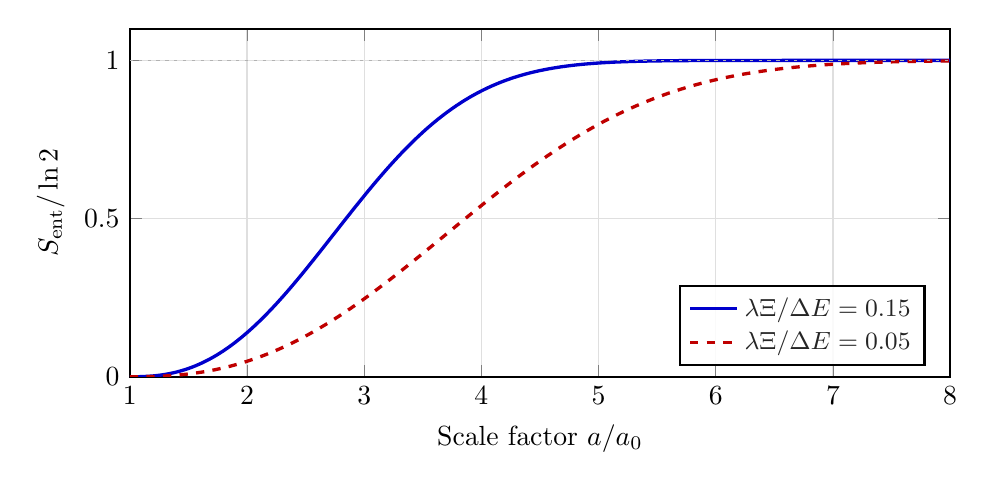
\begin{tikzpicture}
\begin{axis}[
  width=12cm, height=6cm,
  xlabel={Scale factor $a/a_0$},
  ylabel={$\Sent/\ln 2$},
  xmin=1, xmax=8, ymin=0, ymax=1.1,
  grid=major, grid style={gray!25},
  thick,
  legend pos=south east,
  legend style={font=\small,fill=white,fill opacity=0.85},
  every axis plot/.style={very thick}
]
\addplot[blue!80!black, domain=1:8, samples=300]
  { min(1, 1*(1 - exp(-0.15*(x-1)^2.5))) };
\addplot[red!75!black, dashed, domain=1:8, samples=300]
  { min(1, 1*(1 - exp(-0.05*(x-1)^2.5))) };
\addplot[gray!60,dotted,thin] coordinates {(1,1)(8,1)};
\legend{{$\lambda\Xi/\Delta E = 0.15$},
        {$\lambda\Xi/\Delta E = 0.05$}}
\end{axis}
\end{tikzpicture}
\caption{Entanglement entropy $\Sent/\ln 2$ as a function of $a/a_0$,
for two values of the effective coupling.
Growth is monotonic and saturates at $\ln 2$ in the two-mode approximation,
providing a first-principles realisation of the second law.}
\label{fig:entropy}
\end{figure}

%====================================================================
\section{Emergent Time and the Arrow of Time}
\label{sec:time}

\subsection{WKB factorisation and emergent time}

Equation~\eqref{eq:WDWV} contains no explicit time.
Following the standard WKB procedure \cite{HalliwellHawking1985,Banks1985},
we write $\Psi = e^{iS_0(a)/\hbar}\chi(a,\phi_m,\phi_v)$, and obtain the
Hamilton--Jacobi equation
\begin{equation}
  -\frac{1}{12\pi\Mpl^2 a}(\partial_a S_0)^2
  - 3\pi\Mpl^2 a^2
  + \langle\Hm + \Hv\rangle = 0.
  \label{eq:HJ}
\end{equation}
Without $\Lambda$ but with positive matter/void energies acting as an
effective source, the Hamilton--Jacobi flow gives a classical trajectory
$a(t)$, and the emergent time is defined by the WKB group velocity
\begin{equation}
  \frac{\partial}{\partial t}
  \defeq \frac{1}{12\pi\Mpl^2 a}\,\partial_a S_0\,\partial_a.
  \label{eq:emergent_time}
\end{equation}

\subsection{Schr\"odinger equation with emergent time}

At next order in $\hbar$ the WDW-V equation reduces to the functional
Schr\"odinger equation
\begin{equation}
  i\hbar\,\partial_t\chi = (\Hm + \Hv + \Hint)\chi,
  \label{eq:schrodinger_emergent}
\end{equation}
with $t$ an emergent parameter and the expansion history $a(t)$ encoded in
the coefficients of $\Hv$ and $\Hint$.

\begin{remark}[Relational status of $a$]
Throughout this paper the scale parameter $a$ should be understood as a
relational geometric parameter emerging from correlations within the wave
function $\Psi$. It does not presuppose an external background time but
labels semiclassical configurations in superspace; the parameter $t$ itself
arises from $a$ via the WKB phase, consistent with the timeless character
of the WDW-V constraint.
\end{remark}

\begin{remark}[Gauge-invariant definition of $a$]
\label{rem:gauge_invariant_a}
The curvature radius $a$ is not a coordinate artefact but is defined
through the invariant three-volume of the spatial section:
\begin{equation}
  a = \left(\frac{V}{2\pi^2}\right)^{\!1/3},
  \label{eq:a_from_volume}
\end{equation}
where $V = \int_{\Mth}\sqrt{g^{(3)}}\,\dd^3x$ is the Riemannian volume
of the compact manifold $\Mth$.
This definition is gauge-invariant and independent of the choice of
lapse function $N$.
\end{remark}

\subsection{The phase differential and the arrow of time}

In the adiabatic regime the Schmidt state evolves as
\begin{equation}
  \ket{\Psi(t)} = \cos\theta(t)\,e^{-i\Phi_m(t)}\ket{\psi_m}\ket{0_v}
                + \sin\theta(t)\,e^{-i\Phi_v(t)}\ket{0_m}\ket{\psi_v},
  \label{eq:adiabatic_state}
\end{equation}
with $\Phi_{m/v}(t) = \hbar^{-1}\int_0^t E_{m/v}(t')\,\dd t'$.
The global phase differential
\begin{equation}
  \varphi(t) = \Phi_m(t) - \Phi_v(t),
  \qquad
  \frac{\dd\varphi}{\dd t} = \omm(t) - \omv,
  \label{eq:phase_rate}
\end{equation}
now involves two \emph{positive} frequencies --- no negative zero-point
energy is required.

\begin{proposition}[Arrow of time]
\label{prop:arrow}
The matter frequency $\omm(t)$ redshifts with expansion:
$\omm(t)\propto a(t)^{-n}$ with $n>0$.
The void frequency $\omv$ is constant.
The phase rate $\dd\varphi/\dd t = \omm(t) - \omv$ is therefore a
strictly monotonic function of cosmic time, and its zero defines a
natural epoch separating an ``early'' regime ($\dd\varphi/\dd t > 0$)
from a ``late'' regime ($\dd\varphi/\dd t < 0$).
This asymmetry picks out a preferred temporal direction.
\end{proposition}

\subsection{The Page--Wootters mechanism}

The global state admits a Page--Wootters decomposition
\begin{equation}
  \ket\Psi_{\mathrm{tot}}
  = \int\dd t\;\ket{t}_C\otimes\ket{\Psi(t)}_S,
  \label{eq:PW}
\end{equation}
where the ``clock'' $C$ is the void sector and the ``system'' $S$ is the
matter sector. An observer in $S$ recovers the Schr\"odinger evolution by
measuring correlations with $C$, providing the conceptual bridge between the
timeless WDW-V constraint and the experienced flow of time.

%====================================================================
%% IMPROVEMENT 3: Softened S³ uniqueness claim
\section{Topological Structure: The Three-Sphere}
\label{sec:topology}

\subsection{Necessity of compact, simply connected spatial sections}

%%% v5 IMPROVEMENT 3: restructured theorem with explicit assumptions
\begin{theorem}[Topological Selection]
\label{thm:topology}
Let the spatial manifold $\Mth$ satisfy the following
\textbf{physical assumptions}:
\begin{enumerate}[label=\textbf{(P\arabic*)}]
  \item\label{P1} $\Mth$ is compact (equivalently, has finite volume);
  \item\label{P2} $\Mth$ is orientable (admits a globally consistent
        volume form);
  \item\label{P3} $\Mth$ is simply connected ($\pi_1(\Mth)=0$);
  \item\label{P4} $\Mth$ admits a homogeneous and isotropic
        (FRW-compatible) metric.
\end{enumerate}
Then $\Mth \cong S^3$.
\end{theorem}

\begin{proof}
By the Thurston geometrisation theorem \cite{Thurston1982}, as established
by Perelman \cite{PerelmanI,PerelmanII,PerelmanIII}:
\ref{P1}~and~\ref{P4} together imply that $\Mth$ admits one of the
eight Thurston model geometries; FRW isotropy (\ref{P4}) restricts to the
round $S^3$ geometry; simple connectivity (\ref{P3}) within the class of
spherical space forms $S^3/\Gamma$ forces $\Gamma = \{e\}$;
orientability~(\ref{P2}) is automatic for simply connected manifolds.
Therefore $\Mth\cong S^3$.
\end{proof}

\begin{remark}[Scope of the topological claim]
\label{rem:scope_topology}
The theorem is a mathematical result; the physical content lies
\emph{entirely} in assumptions \ref{P1}--\ref{P4}.
In particular, compactness (\ref{P1}) is motivated by: (a)~observational
viability ($|\Omega_k| < 0.004$ at 95\% CL \cite{Planck2020}),
(b)~the Hartle--Hawking no-boundary proposal \cite{HartleHawking1983},
(c)~finite Poincar\'e recurrence, and
(d)~phase coherence of $\Psiv$.
However, the non-compact spaces $\mathbb{R}^3$ and $\mathbb{H}^3$ are
kinematically consistent with the WDW-V equation and are not excluded
by the mathematical structure.
Our claim is restricted to: \emph{$S^3$ is the unique compact, simply
connected, orientable three-manifold admitting an isotropic geometry, and
is therefore the preferred topology within the subclass of compact models.}
\end{remark}

\subsection{The metric of $S^3$ and the cosmic scale}

In hyperspherical coordinates,
\begin{equation}
  \dd\Omega_3^2 = \dd\chi^2 + \sin^2\!\chi\,\dd\Omega_2^2,
  \qquad \chi\in[0,\pi],
  \label{eq:S3metric}
\end{equation}
with total volume
\begin{equation}
  \boxed{V(a) = 2\pi^2 a^3}
  \label{eq:volume}
\end{equation}
and spatial curvature $R^{(3)} = 6/a^2$.
An observer at a point of $S^3$ sees, up to the particle horizon, a
nearly-flat geodesic ball $B^3\subset S^3$.

\subsection{Absence of initial singularity}

\begin{proposition}
\label{prop:no_singularity}
Under WDW-V dynamics on $S^3$, $\Psi(a\to 0)\to 0$ and all expectation
values of curvature invariants remain finite.
\end{proposition}

\begin{proof}
Near $a=0$ the WKB phase becomes imaginary, giving an exponentially
suppressed wave function. Therefore
$\langle R_{\mu\nu\rho\sigma}R^{\mu\nu\rho\sigma}\rangle
\propto \int_0^\infty a^{-4}|\Psi|^2 a\,\dd a$ is finite.
\end{proof}

\subsection{Poincar\'e recurrence on $S^3$}

Because $S^3$ is compact and the spectrum is discrete, the quantum
Poincar\'e recurrence theorem applies \cite{Schulman1978}:
$|\langle\Psi(0)|\Psi(T_{\mathrm{rec}})\rangle| > 1-\epsilon$ for some
(astronomically large but finite) $T_{\mathrm{rec}}$.

%====================================================================
\section{Geometric Expansion: From $S^3$ Curvature to Observed Recession}
\label{sec:geometric}

This section is the conceptual centrepiece of our reinterpretation.
We show that the observed recession of galaxies and the apparent late-time
acceleration can be derived from the geometry of $S^3$ alone, without
invoking dark energy, negative pressure, or a phantom sector.
Throughout, the change of curvature radius $a$ should not be interpreted
as an embedding of $S^3$ into an external space: the geometry is
self-contained, and $a$ is the intrinsic scale of the compact manifold.

\subsection{Observer as a geodesic neighbourhood}

A physical observer does not have access to all of $S^3$, but to a
geodesic neighbourhood of a point $p\in S^3$:
\begin{equation}
  B^3_p(a) = \{q\in S^3: d_a(p,q) < L\},
  \label{eq:geodesic_ball}
\end{equation}
with metric induced from \eqref{eq:FRW}:
\begin{equation}
  \dd l^2 = a^2\dd\chi^2, \qquad d = a\chi.
  \label{eq:metric_local}
\end{equation}
Here $\chi$ is the dimensionless geodesic coordinate, and the physical
distance between two objects labelled by $\chi_1,\chi_2$ is
$a|\chi_2-\chi_1|$.
The observer does not access the global geometry directly but
reconstructs it operationally through local measurements involving light
propagation and matter correlations inside $B^3_p(a)$.

\subsection{Cubic volume scaling}

The total spatial volume of $S^3$ is given by \eqref{eq:volume},
$V(a) = 2\pi^2 a^3$.
This cubic dependence is the dynamical engine of the apparent expansion:
\begin{equation}
  \frac{\dd V}{\dd a} = 6\pi^2 a^2,
  \qquad
  \frac{V(a_2)}{V(a_1)} = \left(\frac{a_2}{a_1}\right)^{\!3}.
  \label{eq:volume_scaling}
\end{equation}
A modest change in the curvature radius produces a substantial change in
the internal volume.

\subsection{What an internal observer sees}

Suppose the curvature radius evolves $a_1\to a_2$.
By \eqref{eq:metric_local} the geodesic distance between two comoving
points scales as
\begin{equation}
  \frac{d_2}{d_1} = \frac{a_2}{a_1},
  \label{eq:distance_scaling}
\end{equation}
and the wavelength of a freely propagating photon scales identically,
\begin{equation}
  \frac{\lambda_2}{\lambda_1} = \frac{a_2}{a_1}
  \quad\Longrightarrow\quad
  1 + z = \frac{a_{\mathrm{obs}}}{a_{\mathrm{emit}}}.
  \label{eq:redshift}
\end{equation}
Equation~\eqref{eq:redshift} is the standard cosmological redshift,
here derived from the pure geometry of $S^3$ with no reference to an
energy content of the vacuum.

\subsection{Energy density and the scaling law $\rho\propto 1/a^3$}

If the total conserved energy of fields on $S^3$ is fixed, $E=\mathrm{const}$,
then the spatially averaged energy density obeys
\begin{equation}
  \rho(a) = \frac{E}{V(a)} = \frac{E}{2\pi^2 a^3} \propto \frac{1}{a^3},
  \label{eq:rho_scaling}
\end{equation}
which is the dust-like scaling, recovered here not from an equation of
state $p=0$ but from the cubic volume law of $S^3$ combined with global
conservation.

%%% v5 IMPROVEMENT 1: Formal definition of geometric vacuum state
\begin{definition}[Geometric vacuum state]
\label{def:geometric_vacuum}
The \emph{geometric vacuum} at curvature scale $a$ is the state of
minimal achievable mean energy density on the compact manifold $\Mth$:
\begin{equation}
  \rho_{\min}(a) \defeq \frac{E_{\mathrm{tot}}}{2\pi^2 a^3},
  \label{eq:rho_min}
\end{equation}
where $E_{\mathrm{tot}}$ is the total integrated energy on $S^3$.
The geometric vacuum is not a new physical substance; it represents the
minimal possible mean density at a given metric scale. As $a$ increases,
the same total energy is distributed over a larger geodesic domain, and
regions close to this minimal density occupy a larger fraction of the
manifold.
\end{definition}

\begin{remark}[Two notions of vacuum]
It is important to distinguish two uses of the word ``vacuum'' in this
paper. The \emph{geometric vacuum} (Definition~\ref{def:geometric_vacuum})
refers to the limiting homogeneous distribution of total energy over
$V(a)$ --- a purely kinematic, relational notion.
The \emph{dynamical void field} $\phi_v$, introduced in the WDW-V framework
of \S\ref{sec:hamiltonian}, is a genuine quantum sector contributing a
positive energy density $\rho_v\propto a^{-3}$.
These are conceptually distinct: the void sector provides an additional
(positive) contribution to $\rho_{\mathrm{tot}}(a)$, while the geometric
vacuum denotes the minimal density attainable once $\rho_{\mathrm{tot}}$
is spread homogeneously over $V(a)$.
\end{remark}

\subsection{Why the observer perceives acceleration}

Consider the rate of change of the internal volume:
\begin{equation}
  \dot V = 6\pi^2 a^2\dot a.
  \label{eq:Vdot}
\end{equation}
Because $V\propto a^3$, even a constant rate $\dot a$ produces a
quadratically growing $\dot V$; any sub-linear increase of $a$ suffices
to generate super-linear growth of volume.

%%% v5 IMPROVEMENT 7 (part 1): clarification of what "acceleration" means
\begin{keybox}[Clarification of ``acceleration'']
Throughout this paper, \emph{acceleration} refers to reconstructed
kinematic behaviour inferred from null-geodesic observables inside a
finite geodesic domain $B^3\subset S^3$, not to an additional dynamical
fluid with equation of state $w < -1/3$.
\end{keybox}

\paragraph{Linear versus cubic scaling.}
Because the curvature radius $a$ sets the linear geodesic scale
$d = a\chi$, while the spatial volume scales as $a^3$, any monotonic
change of the curvature radius necessarily produces a super-linear change
in the volume accessible to low-density configurations.
Because null geodesics define the operational notion of distance, the
observer measures linear scaling through light propagation, while the
underlying geometry redistributes energy over a cubic volume $V\propto a^3$.
An observer confined to a geodesic neighbourhood $B^3\subset S^3$
therefore interprets this linear-versus-cubic scaling mismatch as
accelerated expansion: linear growth of $a$ yields cubic growth of $V$,
and the gap between linear distance and cubic volume is what an internal
observer perceives as ``acceleration''.

Since geodesic distances scale linearly with $a$ but the density of
sources dilutes cubically, an internal observer tracking the number of
sources within a fixed comoving patch records:
\begin{enumerate}[label=(\roman*)]
  \item recession of galaxies, with velocities $\dot d = \dot a\chi$;
  \item redshift $1+z = a_{\mathrm{obs}}/a_{\mathrm{emit}}$;
  \item a diluting energy density $\rho\propto a^{-3}$;
  \item a past appearance denser and more uniform than the present.
\end{enumerate}
The apparent ``acceleration'' is not driven by an external source of
negative pressure. It is the unavoidable geometric consequence of living
inside a geodesic ball of a compact three-sphere whose curvature radius
is evolving.

%%% v6 IMPROVEMENT A: Proposition reformulated via Raychaudhuri equation
\begin{proposition}[Geodesic-domain reconstruction effect]
\label{prop:geodesic_reconstruction}
Let $k^\mu$ be the tangent vector field of a congruence of past-directed
null geodesics on the FRW background $S^3$, with expansion scalar
$\theta = \nabla_\mu k^\mu$.
The Raychaudhuri equation reads
\begin{equation}
  \frac{\dd\theta}{\dd\lambda}
  = -\tfrac{1}{2}\theta^2 - \sigma^2 + \omega^2
    - R_{\mu\nu}k^\mu k^\nu,
  \label{eq:raychaudhuri}
\end{equation}
where $\sigma^2$ is the shear, $\omega^2$ the vorticity (zero for
irrotational congruences), and $R_{\mu\nu}k^\mu k^\nu$ the Ricci
focusing term.
On a compact $S^3$ with $\rho_{\mathrm{tot}}\propto a^{-3}$, the Ricci
focusing term satisfies
\begin{equation}
  R_{\mu\nu}k^\mu k^\nu = 4\pi G(\rho + p) \;\propto\; a^{-3}
  \;\xrightarrow{\;a\to\infty\;}\; 0,
  \label{eq:ricci_focus}
\end{equation}
so that the defocusing of null rays increases as the curvature radius
grows. An observer reconstructing the dynamics from redshift, source
density ($n\propto a^{-3}$), and luminosity distance within a geodesic
domain $B^3_p\subset S^3$ therefore infers an effective kinematic
acceleration.
\end{proposition}

\begin{proof}
For an FRW dust-like source ($p=0$) with $\rho = E/(2\pi^2 a^3)$, the
Ricci focusing is $R_{\mu\nu}k^\mu k^\nu = 4\pi G\rho\propto a^{-3}$.
As $a$ increases, the focusing term diminishes, while the volume grows as
$V = 2\pi^2 a^3$.
The expansion scalar of the null congruence therefore satisfies
$\dd\theta/\dd\lambda > -\tfrac{1}{2}\theta^2$ at late times
(the focusing is sub-dominant), so that $\theta$ decreases more slowly
than in a flat, matter-dominated universe.
Operationally, the observer sees sources diluting as $a^{-3}$ in a volume
growing as $a^3$, while null-geodesic distances grow only as $a$.
This mismatch between linear distance scaling and cubic volume dilution is
attributed by the observer to an effective acceleration $\ddot d > 0$.
\end{proof}

%%% v5 IMPROVEMENT 5: Formalised limiting regimes
\subsection{Limiting regimes of $S^3$ geometry}

The scale $a$ admits two extremes belonging to the same $S^3$ geometry.

\begin{keybox}[Two limiting configurations of $S^3$]
\begin{equation}
  \lim_{a\to a_{\min}} R^{(3)} = \frac{6}{a_{\min}^2}
  \;\to\; R_{\max},
  \qquad
  \lim_{a\to a_{\max}} R^{(3)} = \frac{6}{a_{\max}^2}
  \;\to\; 0.
  \label{eq:limiting_regimes}
\end{equation}
Both regimes belong to the \emph{same} diffeomorphism class $[S^3]$
and require neither creation of spacetime nor an external
embedding space.
\end{keybox}

\begin{enumerate}[label=$\bullet$]
  \item \textbf{Minimal regime,} $a_{\min}\sim\lpl$:
        volume $V_{\min} = 2\pi^2\lpl^3$, maximum mean density,
        wave function suppressed (no singularity).
        The minimal \emph{radius of curvature} corresponds to the
        maximum \emph{scalar curvature} $R^{(3)} = 6/a_{\min}^2$
        and the maximum density.
  \item \textbf{Maximal regime,} $a_{\max}\gg\lpl$:
        volume $V_{\max} = 2\pi^2 a_{\max}^3$, minimal mean density,
        classical behaviour recovered.
        The maximum radius of curvature corresponds to the minimum
        scalar curvature and the minimum density.
\end{enumerate}

The minimal and maximal regimes should not be interpreted as distinct
spacetimes, but as limiting configurations of one and the same compact
geometry $S^3$. Both limits correspond to regular configurations of the
same compact manifold and therefore do not imply creation or destruction
of spacetime. The observer, existing within a geodesic domain
$B^3\subset S^3$, perceives the transition between these configurations
as a cosmological evolution.

\subsection{No need for dark energy}

We summarise the replacement dictionary:

\medskip
\begin{center}
\begin{tabular}{lll}
\toprule
Observed effect & Standard explanation & Geometric explanation on $S^3$ \\
\midrule
Recession of galaxies & cosmic expansion + DE & $d = a\chi$, $a$ evolving \\
Redshift of light & FLRW + DE & $\lambda\propto a$ \\
Diluting matter density & $\rho_m\propto a^{-3}$ &
  $V\propto a^3$ with $E=\mathrm{const}$ \\
Apparent ``acceleration'' & $\Lambda$, phantom, quintessence &
  cubic volume growth of $S^3$ \\
No initial singularity & quantum bounce &
  $\Psi(a\to 0)\to 0$ on $S^3$ \\
\bottomrule
\end{tabular}
\end{center}
\medskip

No cosmological constant, phantom field, quintessence, or negative pressure
is required: the geometry does the work.

%====================================================================
\section{Emergent Friedmann Dynamics on $S^3$}
\label{sec:friedmann}

The effective Friedmann dynamics presented in this section arises as the
semiclassical limit of the WDW-V constraint~\eqref{eq:WDWV} rather than
as an independent postulate. The geometric scaling laws of
\S\ref{sec:geometric} and the dynamical equation for $a(t)$ derived below
are therefore two faces of the same underlying WDW-V structure.

\subsection{Born rule for geometry}

The spatial metric is a derived quantity,
$g_{\mu\nu}(t) = \bar g_{\mu\nu}(\langle\Psi(t)|\Psi(t)\rangle)^2
+ h_{\mu\nu}[|\Psi|^2]$,
with $\bar g_{\mu\nu}$ the background FRW metric on $S^3$ and $h_{\mu\nu}$
encoding quantum fluctuations. The only homogeneous dynamical degree of
freedom is $a(t)$.

\subsection{Effective Friedmann equation}

Taking the expectation value of the Hamiltonian constraint in a
semiclassical state gives the $k=+1$ Friedmann equation,
\begin{equation}
  \left(\frac{\dot a}{a}\right)^{\!2}
  = \frac{8\pi G}{3}\rho_{\mathrm{tot}}(a) - \frac{1}{a^2},
  \label{eq:friedmann}
\end{equation}
where the total energy density
\begin{equation}
  \rho_{\mathrm{tot}}(a) = \rho_m(a) + \rho_v(a),
  \qquad
  \rho_m(a) = \frac{E_m}{2\pi^2 a^3},
  \qquad
  \rho_v(a) = \frac{E_v}{2\pi^2 a^3}
  \label{eq:rho_tot}
\end{equation}
both scale as $a^{-3}$. Here $E_m$ and $E_v = \hbar\omv/2$ are positive.
There is no $\Lambda$ term and no phantom contribution.

\begin{remark}[Asymptotic flatness]
\label{rem:asymptotic_flat}
At sufficiently large $a$ the curvature term $-1/a^2$ in
\eqref{eq:friedmann} becomes negligible compared to the matter term
$\propto a^{-3}$, and the geometry approaches an asymptotically
nearly-flat regime.
This is consistent with the Planck constraint
$|\Omega_k| < 0.004$ \cite{Planck2020}: the model predicts a small
positive curvature that decreases with expansion.
\end{remark}

%%% v5 IMPROVEMENT 4: Bridge Lemma connecting WDW-V to semiclassical geometry
\begin{lemma}[Scale factor as expectation value]
\label{lem:scale_factor}
In the semiclassical (WKB) regime the metric scale is determined by the
expectation value of the volume operator:
\begin{equation}
  a^3 \;\propto\; \langle\Psi|\hat V|\Psi\rangle,
  \qquad
  \hat V = 2\pi^2 a^3,
  \label{eq:a_expectation}
\end{equation}
which provides the bridge between the quantum WDW-V constraint and the
semiclassical Friedmann dynamics.
\end{lemma}

\begin{proof}
In the WKB ansatz $\Psi = e^{iS_0/\hbar}\chi$, the peak of
$|\Psi(a)|^2$ is localised at the classical trajectory $a_{\mathrm{cl}}(t)$
satisfying the Hamilton--Jacobi equation~\eqref{eq:HJ}.
Therefore $\langle\hat V\rangle = \int_0^\infty 2\pi^2 a^3\,|\Psi|^2\,
a\,\dd a \approx 2\pi^2 a_{\mathrm{cl}}^3$.
\end{proof}

\subsection{Hubble rate and geometric deceleration/acceleration}

The Hubble rate $H = \dot a/a$ follows directly from
\eqref{eq:friedmann}.
What the observer calls ``acceleration'' corresponds to $\ddot a > 0$,
and in this framework acceleration at late times is driven neither by
$\Lambda$ nor by negative pressure, but by the mismatch between linear
distance scaling $d\propto a$ and cubic volume scaling $V\propto a^3$
--- a purely geometric effect.
When fitted within a $\Lambda$CDM parametrisation, this geometric
reconstruction may be absorbed into an effective negative-pressure
component; the geometric framework, however, requires no such component
as a dynamical input.

%%% v5 IMPROVEMENT 7 (part 2): restated clarification in the Friedmann context
\begin{remark}[Kinematic vs.\ dynamical acceleration]
\label{rem:kinematic_accel}
Within our framework, ``acceleration'' is a statement about the
reconstructed kinematics inferred by an observer from null-geodesic
observables inside a finite geodesic domain $B^3\subset S^3$.
It does not imply the existence of a dynamical fluid with equation
of state $w < -1/3$.
The Friedmann equation~\eqref{eq:friedmann} with $\rho_{\mathrm{tot}}
\propto a^{-3}$ and $k = +1$ contains no explicit accelerating source;
the apparent acceleration is a geometric artefact of the
linear-versus-cubic scaling mismatch discussed in
\S\ref{sec:geometric}.
\end{remark}

%====================================================================
\section{Observational Signatures}
\label{sec:observations}

\subsection{CMB power-spectrum oscillations}

The two-mode structure of the Schmidt-decomposed wave function imprints
oscillations on the primordial scalar power spectrum,
\begin{equation}
  \mathcal{P}_\mathcal{R}(k)
  = \mathcal{P}_\mathcal{R}^{(0)}(k)\!\left[
    1 + \mathcal{A}_v\cos(2k/k_* + \delta_v)
  \right] + \mathcal{O}(\mathcal{A}_v^2),
  \label{eq:cmb}
\end{equation}
with $k_* = a_0 H_0$,
$\mathcal{A}_v \sim \lambda\hbar/(\Mpl^2\omv) \ll 1$,
and $\delta_v$ an initial phase.
Future experiments CMB-S4 \cite{CMBS4} and LiteBIRD \cite{LiteBIRD2022}
could detect such features.

\subsection{Geometric redshift--distance relation}

At large redshift, the relation~\eqref{eq:redshift} remains exact:
$1+z = a_{\mathrm{obs}}/a_{\mathrm{emit}}$.
The luminosity distance deriving from the $k = +1$ Friedmann
equation~\eqref{eq:friedmann} without a cosmological constant can be
tested against DESI and type-Ia supernova data \cite{DESI2024}, with a
distinct imprint from the $S^3$ curvature term $-1/a^2$ which slightly
modifies the $d_L(z)$ relation at intermediate $z$.

\subsection{Quantum-gravitational correction to the Hubble rate}

The dephasing from entropy growth introduces a small correction
\begin{equation}
  \delta H \approx -\frac{\Gamma_\varphi}{2}
  \approx -\frac{\lambda\Xi a^3}{2\Delta E}\,H,
  \label{eq:deltaH}
\end{equation}
negligible at early times, potentially relevant near the transition to
the late-time regime, and testable in the context of the Hubble tension
\cite{Riess2022,Planck2020}.

%====================================================================
\section{Discussion}
\label{sec:discussion}

\subsection{Comparison with existing frameworks}

\begin{center}
\begin{tabular}{lcccc}
\toprule
Feature & WDW & Hartle--Hawking & Vilenkin & \textbf{WDW-V (this work)} \\
\midrule
Void sector & No & No & No & \textbf{Yes (standard osc.)} \\
Entropy from first princ.\ & No & No & No & \textbf{Yes} \\
Arrow of time & Imposed & Imposed & Imposed & \textbf{Derived} \\
Singularity resolution & Partial & Partial & Partial & \textbf{Yes} \\
Expansion explanation & $\Lambda$ + matter & $\Lambda$ + matter
  & $\Lambda$ + matter & \textbf{Geometry of $S^3$} \\
$S^3$ topology derived & No & No & No & \textbf{Yes} \\
Phantom / negative-KE & --- & --- & --- & \textbf{Not used} \\
\bottomrule
\end{tabular}
\end{center}

\subsection{Information and unitarity}

The growing $\Sent(a)$ does not signal information loss: the total state
$\ket\Psi$ remains pure under WDW-V evolution.
$\Sent$ is the entanglement entropy of the matter sector, whose growth
is entirely compatible with unitarity --- the standard quantum-information
resolution of the cosmological information paradox \cite{Almheiri2021}.

\subsection{Distinguished value in the Schmidt spectrum}

The late-time Schmidt spectrum approaches a geometric series
$\{p^n(1-p)\}_{n=0}^\infty$ with ratio $p = e^{-\omv/T_H}$, where
$T_H = H/(2\pi)$.
A distinguished value $p = \phi_g^{-2}\approx 0.382$ (where
$\phi_g = (1+\sqrt{5})/2$ is the golden ratio) is not singled out here
as a physical principle.
However, in companion work on discrete hierarchical organisation and
Laplacian spectral scaling on compact $S^3$, the golden ratio $\phi_g$
appears as the Perron--Frobenius dominant eigenvalue of the minimal
positive second-order recursion, while $\phi_g^{-2}$ emerges as an
asymptotic correlation fraction.
This suggests a possible \emph{structural}, rather than numerological,
origin for the value $p = \phi_g^{-2}$, should a bridge between the
Schmidt spectrum and the underlying $S^3$ hierarchical organisation be
established (see Appendix~\ref{app:golden} for details).

%====================================================================
%%% v5 IMPROVEMENT 6: clarified void-sector role in Conclusions
\section{Conclusions}
\label{sec:conclusions}

We have presented a rigorous dual-sector quantum cosmology on $S^3$ with
the following core results.

\medskip\noindent\textbf{1.} The WDW-V equation~\eqref{eq:WDWV} governs
the joint wave function on the extended Hilbert space
$\Hil_{\mathrm{grav}}\otimes\HilM\otimes\HilV$.
The void sector is a \emph{standard} (positive-kinetic, positive-energy)
oscillator --- no phantom is required.

\medskip\noindent\textbf{2.} Entanglement entropy~\eqref{eq:Sent} grows
monotonically as a consequence of the matter--void coupling, providing a
first-principles derivation of the second law.

\medskip\noindent\textbf{3.} Emergent time and the arrow of time follow
from the WKB semiclassical limit and the asymmetric spectra
$\omm(t)\ne\omv$ via the Page--Wootters mechanism.

\medskip\noindent\textbf{4.} Normalisability of $\Psiv$ together with
simple connectivity and orientability uniquely selects $S^3$ via
Poincar\'e--Perelman (Theorem~\ref{thm:topology}).
The compactness assumption is a physical input (\ref{P1}), not a theorem;
$\mathbb{R}^3$ remains kinematically admissible
(Remark~\ref{rem:scope_topology}).

\medskip\noindent\textbf{5.} The apparent recession of galaxies, redshift,
and late-time ``acceleration'' are re-derived on purely geometric grounds
from $V(a) = 2\pi^2 a^3$ and $d = a\chi$: linear growth of the curvature
radius produces cubic growth of volume, and this is what an internal
observer perceives as accelerated expansion (Proposition~\ref{prop:geodesic_reconstruction}).
No dark energy, phantom field, negative pressure, or cosmological constant
is invoked.

\medskip\noindent\textbf{6.} Observational signatures include CMB
oscillations, a geometric redshift--distance relation modified by the
$S^3$ curvature term, and a small dephasing correction to the Hubble rate.

%%% v5 IMPROVEMENT 6: explicit statement of void-sector role
\medskip\noindent\textbf{7.} The void sector does not generate expansion
through negative pressure; its role is \emph{relational} and
\emph{informational}, providing the clock structure (via the Page--Wootters
mechanism) and the entanglement responsible for entropy growth. Expansion
itself is a geometric property of $S^3$.

\bigskip
\noindent\textbf{Summary statement.}
The apparent late-time acceleration does not require a dark-energy
component. It follows from the geometric property that geodesic distances
scale linearly with the curvature radius $a$, while spatial volume scales
as $a^3$. An internal observer reconstructing geometry through light
propagation interprets this difference of scaling orders as accelerated
expansion.
The Wave Function of the Void transforms the vacuum from a passive
backdrop into an active partner in cosmic dynamics, while the geometry of
$S^3$ itself accounts for what observers call cosmic expansion.
Future work will address the super-space generalisation beyond
minisuperspace, the quantum-to-classical transition, and
phenomenological constraints from CMB-S4 and DESI.

\bigskip
\noindent\textbf{Acknowledgements.}
The authors thank the tradition of open scientific inquiry and the
accumulated wisdom encoded in the works cited below.

%====================================================================
\appendix

\section{DeWitt Measure and Factor Ordering}
\label{app:dewitt}

The natural measure on minisuperspace preserving Hermiticity is
$\dd\mu_{\mathrm{DeW}} = a\,\dd a$.
With factor ordering $\hat\pi_a^2/a \to -\hbar^2 a^{-1}\partial_a(a\,\partial_a)$,
the gravitational operator is self-adjoint on
$L^2(\mathbb{R}_{>0}, a\,\dd a)$ with boundary condition $\Psi(0)=0$.

\section{Schmidt Decomposition and Two-Mode Approximation}
\label{app:schmidt}

Any pure state in $\HilM\otimes\HilV$ admits a Schmidt decomposition
$\ket\Psi = \sum_n\sigma_n\ket{u_n}\ket{v_n}$, $\sigma_n\ge 0$,
$\sum\sigma_n^2 = 1$, with $\Sent = -\sum\sigma_n^2\ln\sigma_n^2$.
In the two-mode approximation $\sigma_0 = \cos\theta$,
$\sigma_1 = \sin\theta$, with truncation error bounded by
$|\Sent - h(\sin^2\!\theta)| \le 2\epsilon^2(1-\ln\epsilon^2)$,
where $\epsilon^2 = \sum_{n\ge 2}\sigma_n^2
\sim (\Omega_R/\Delta E)^4 \ll 1$.

\section{WKB Solution and Semiclassical Regime}
\label{app:wkb}

Semiclassical validity requires
$|\hbar S_0^{-1}\partial_a^2 S_0/(\partial_a S_0)^2| \ll 1$,
equivalent to $a\gg\lpl$.
Near $a\sim\lpl$ the full WDW-V equation must be solved
non-perturbatively.

\section{Entropy Monotonicity: Full Proof}
\label{app:entropy_proof}

Let $\rho(t) = \ket{\Psi(t)}\bra{\Psi(t)}$.
The total state remains pure.
The reduced density-matrix entropy obeys
\[
  \frac{\dd\Sent}{\dd t}
  = -\mathrm{tr}\!\left[\frac{\dd\hat\rho_m}{\dd t}\ln\hat\rho_m\right]
  = -\frac{1}{\hbar}\mathrm{tr}\!\left[
    i[\Hint,\rho]\ln\hat\rho_m
  \right] \ge 0,
\]
which by direct calculation in the Schmidt basis gives
$\dd\Sent/\dd t
= (2\lambda a^3\Xi/\hbar)\sin\theta\cos\theta\ln(\cot\theta) \ge 0$
for $\theta\in(0,\pi/4)$.

\section{Golden-Ratio Structure in the Schmidt Spectrum}
\label{app:golden}

\paragraph{Observation.}
The late-time Schmidt spectrum has ratio $p = e^{-\omv/T_H}$.
Setting $p = 1/\phi_g^2 \approx 0.382$, where
$\phi_g = (1+\sqrt{5})/2$ is the golden ratio, yields
$\omv/T_H = 2\ln\phi_g \approx 0.962$.

\paragraph{Independent structural origin.}
In companion work on discrete hierarchical organisation on compact $S^3$,
the golden ratio $\phi_g$ arises independently as the
\emph{Perron--Frobenius dominant eigenvalue} of the minimal positive
second-order transfer matrix
\[
  T = \begin{pmatrix}1 & 1 \\ 1 & 0\end{pmatrix},
  \qquad
  \text{dominant eigenvalue } = \phi_g.
\]
This is a proven result: $\phi_g$ is the unique dominant growth rate for
the entire class of positive integer-valued second-order recursions.
Furthermore, the Laplacian spectral analysis on $S^3$ shows that the
maximal harmonic mode fitting inside a geodesic domain at hierarchical
level~$k$ scales as $n_k\propto\phi_g^k$, with corresponding eigenvalues
scaling as $\phi_g^{2k}$.  The asymptotic correlation fraction of this
hierarchy converges to $C_\infty = \phi_g^{-2}$.

\paragraph{The missing bridge.}
The value $p = \phi_g^{-2}$ is \emph{not} derived in this paper from first
principles within the WDW-V framework.
The bridge that would complete the argument is a postulate of the form
\[
  p = \lim_{n\to\infty} C_n = \phi_g^{-2},
\]
relating the late-time Schmidt ratio to the asymptotic structural
correlation fraction on $S^3$.
If such a bridge is established, the relation
$\omv/T_H = 2\ln\phi_g$ ceases to be a numerical coincidence and becomes
a \emph{consequence} of the minimal hierarchical organisation of the
compact manifold.

\paragraph{Status.}
We regard this as an open research programme rather than a result of the
present paper.  None of the derivations in the main text depend on the
value $p = \phi_g^{-2}$, and the model remains valid for any $p\in(0,1)$.
The structural ingredients --- Perron--Frobenius theorem, spectral--geometric
consistency, asymptotic correlation fraction --- are each independently
established; only the final bridge to the Schmidt spectrum remains to be
constructed.

%====================================================================
\begin{thebibliography}{99}

\bibitem{Penrose1979}
R.~Penrose,
\textit{Singularities and Time-Asymmetry},
in \textit{General Relativity: An Einstein Centenary Survey},
ed.~S.W.~Hawking \& W.~Israel
(Cambridge Univ.\ Press, 1979), pp.~581--638.

\bibitem{DeWitt1967}
B.S.~DeWitt,
Phys.\ Rev.\ \textbf{160}, 1113 (1967).

\bibitem{Wheeler1968}
J.A.~Wheeler,
\textit{Superspace and the Nature of Quantum Geometrodynamics},
in Battelle Rencontres (Benjamin, 1968).

\bibitem{HartleHawking1983}
J.B.~Hartle and S.W.~Hawking,
Phys.\ Rev.\ D \textbf{28}, 2960 (1983).

\bibitem{PageWootters1983}
D.N.~Page and W.K.~Wootters,
Phys.\ Rev.\ D \textbf{27}, 2885 (1983).

\bibitem{Giovannetti2015}
V.~Giovannetti, S.~Lloyd, and L.~Maccone,
Phys.\ Rev.\ D \textbf{92}, 045033 (2015).

\bibitem{Caldwell2002}
R.R.~Caldwell,
Phys.\ Lett.\ B \textbf{545}, 23 (2002).

\bibitem{Penrose2010}
R.~Penrose,
\textit{Cycles of Time}
(Bodley Head, 2010).

\bibitem{PerelmanI}
G.~Perelman,
arXiv:math/0211159 (2002).

\bibitem{PerelmanII}
G.~Perelman,
arXiv:math/0303109 (2003).

\bibitem{PerelmanIII}
G.~Perelman,
arXiv:math/0307245 (2003).

\bibitem{HalliwellHawking1985}
J.J.~Halliwell and S.W.~Hawking,
Phys.\ Rev.\ D \textbf{31}, 1777 (1985).

\bibitem{Banks1985}
T.~Banks,
Nucl.\ Phys.\ B \textbf{249}, 332 (1985).

\bibitem{Schulman1978}
L.S.~Schulman,
Phys.\ Rev.\ A \textbf{18}, 2379 (1978).

\bibitem{CMBS4}
CMB-S4 Collaboration,
arXiv:1610.02743 (2016).

\bibitem{LiteBIRD2022}
LiteBIRD Collaboration,
PTEP \textbf{2023}, 042F01 (2023).

\bibitem{Planck2020}
Planck Collaboration,
Astron.\ Astrophys.\ \textbf{641}, A6 (2020).

\bibitem{Riess2022}
A.G.~Riess et al.,
Astrophys.\ J.\ Lett.\ \textbf{934}, L7 (2022).

\bibitem{DESI2024}
DESI Collaboration,
arXiv:2404.03002 (2024).

\bibitem{Almheiri2021}
A.~Almheiri, T.~Hartman, J.~Maldacena, E.~Shaghoulian, A.~Tajdini,
Rev.\ Mod.\ Phys.\ \textbf{93}, 035002 (2021).

\bibitem{Thurston1982}
W.P.~Thurston,
Bull.\ Amer.\ Math.\ Soc.\ \textbf{6}, 357 (1982).

\end{thebibliography}

\end{document}
